\section{Sofwarearchitektur}
Im folgenden werden die einzelnen Bestandteile der Sofware beschrieben. Die Abbildung veranschaulicht die Zusammenhänge. 
\begin{figure}[htb]
	\centering
		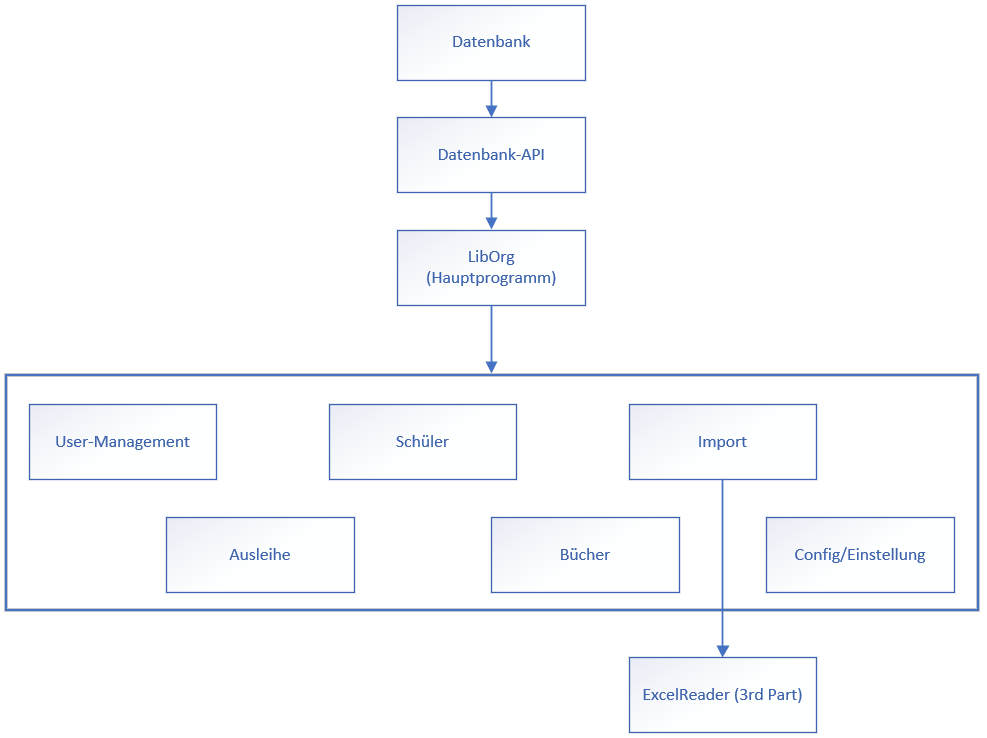
\includegraphics[width=0.90\textwidth]{figures/architecture.png}
	\caption{Die Architektur der Software}
	\label{fig:Architektur}
\end{figure}

\subsection{Datenbank}
Alle anfallenden Daten werden in einer SQLite Datenbank gespeichert. Hierfür wurden die folgenden Tabellen angelegt:
\begin{itemize}
\item BookTable \newline
bildet die im Programm verfügbaren Bücher ab \newline
primary Key: isbn -> ISBN Nummer des Buches \newline
weitere Werte: title -> Buchtitel, subtitle -> Untertitel, publisher -> Verlag, author -> Autor, subject -> Fach, grade -> Klassenstufe, edition -> Auflage, price -> Preis, stock -> auf Lager, available -> verfügbar, comment -> Kommentar, stocktakingCount -> Inventuranzahl, stocktakingDate -> Inventurdatum
\item ClassTable \newline
Klassen, sowie Fächer
\item LendingTable \newline 
Ausleihen 
\item ReturnTable \newline
Rückgaben
\item StudentClassTable \newline 
bildet den Zusammenhang zwsichen Schülern und Klassen ab 
\item StudentTable  \newline
Schüler 
\item UserTable  \newline
Benutzer 
\end{itemize} 
 

\subsection{Datenbank\-API}
Die Datenbank-API dient der Interaktion des C++ Hauptprogramms mit der SQLite Datenbank. Sie stellt alle benötigte Funktionen bereit, welche vom Hauptprogramm benötigt werden. Der Zugriff auf die Datenbank erfolgt ausschließlich über die Datenbank\-API.


\subsection{Hauptanwendung - LibOrg}
Die Grundanwendung(Liborg) stellt das Hauptfenster, das Programmmenü, die  Hilfe, sowie die obere Menüleiste bereit. Über das Programmmenü, kann man die Einstellunge, den Import, die Benutzerverwaltung, den Benutzerwechsel sowie die Backup-Wiederherstellung erreichen. Alle weiteren Funktionen werden über die Reiter der Grundanwendung aufgerufen. 
\begin{figure}[H]
	\centering
		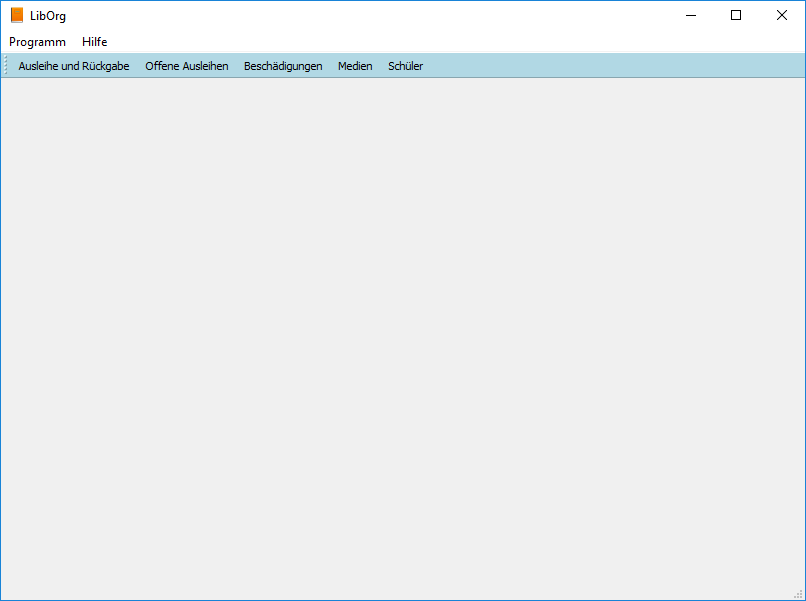
\includegraphics[width=0.70\textwidth]{figures/Liborg.png}
	\caption{LibOrg - die Grundanwendung}
	\label{fig:Mainwindow}
\end{figure}


\subsubsection{Benutzerverwaltung}
Die Benuterverwaltung erreicht man über das das den Menüpunkt "Programm" -> Benutzerverwaltung. Dort werden die Benutzer mit ihren Passwörtern und ihren Berechtigungen verwaltet. Sowie neue Benutzer angelegt und alte gelöscht.
\begin{figure}[H]
	\centering
		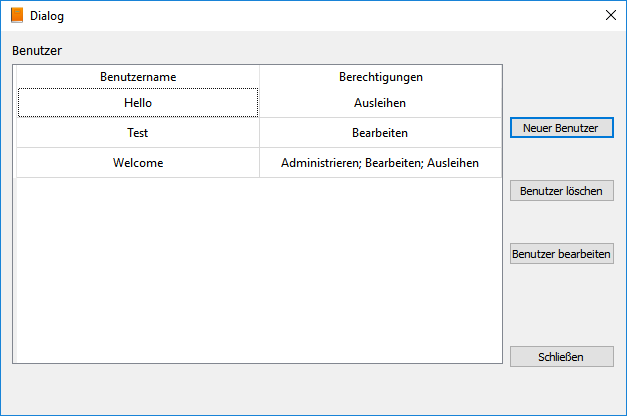
\includegraphics[width=0.70\textwidth]{figures/usermanagement.png}
	\caption{Die Benutzerverwaltung}
	\label{fig:usermanagement}
\end{figure}


\subsubsection{Ausleihe}
Die Ausleihen werden über den Reiter "Ausleihe und Rückgabe" in der Grundanwendung aufgerufen. Hier werden alle ausgeliehene Bücher mit zugehörigem Schüler gespeichert und verwaltet.
\begin{figure}[H]
	\centering
		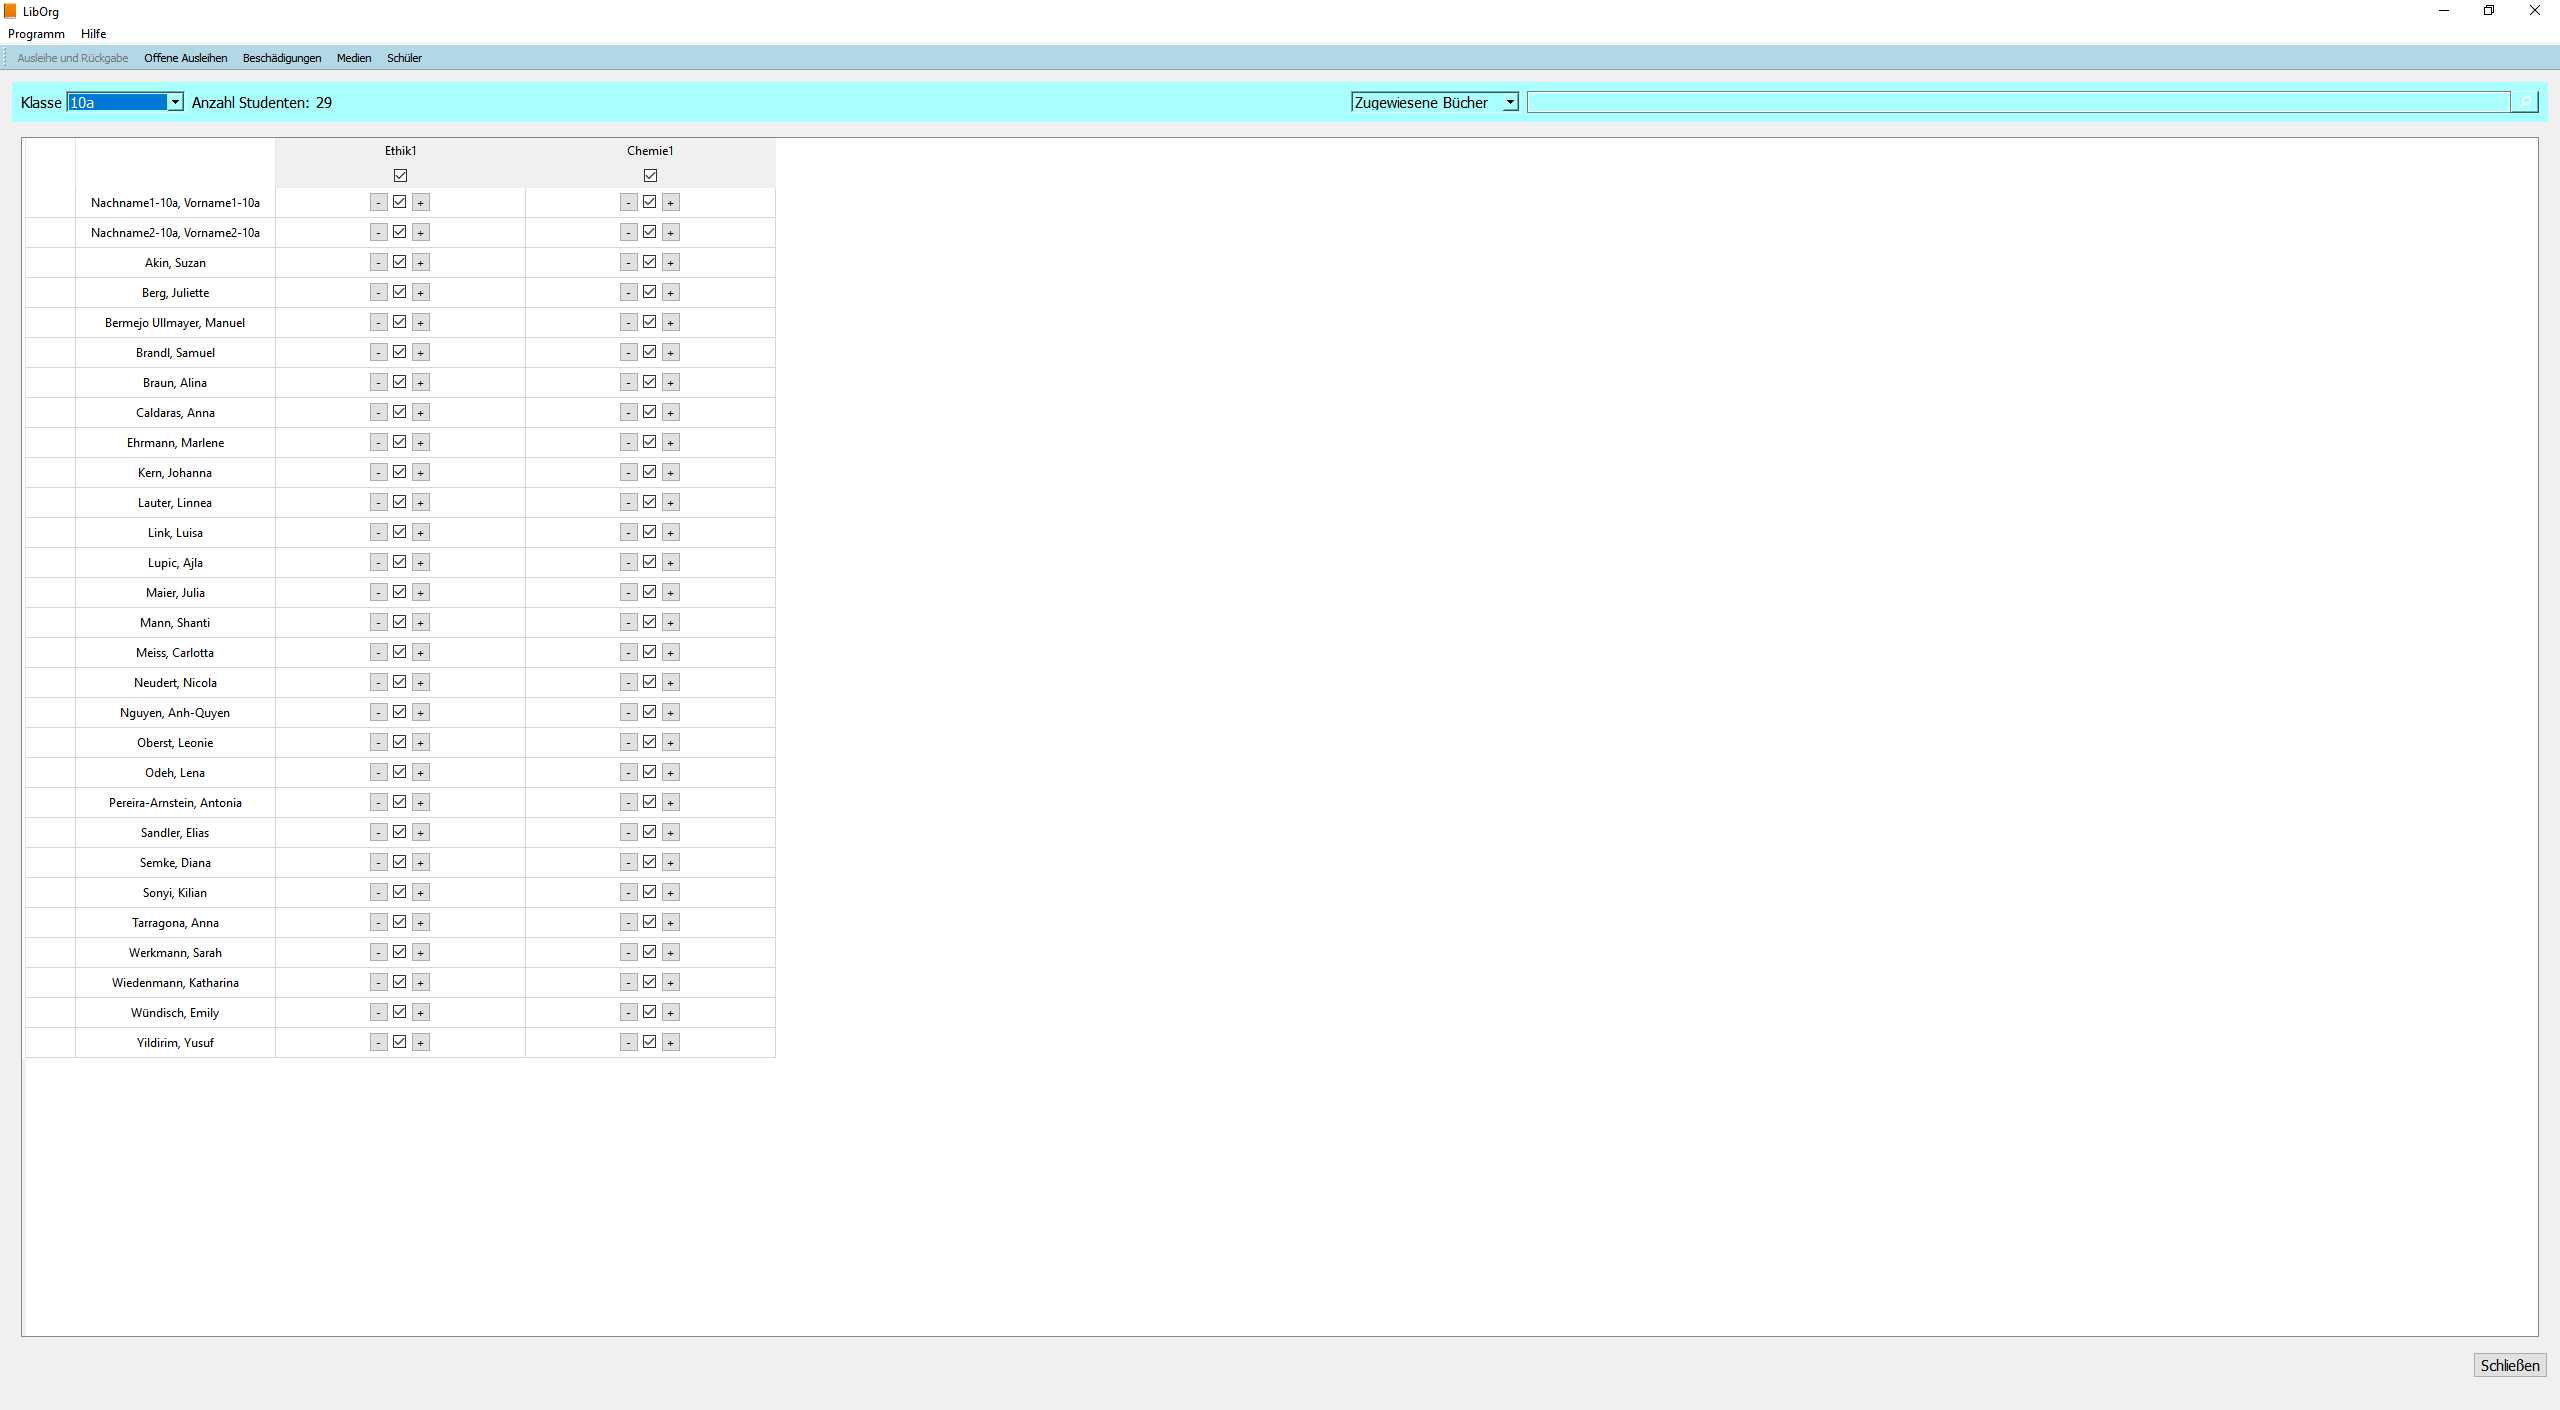
\includegraphics[width=0.70\textwidth]{figures/lendings.png}
	\caption{Ausleihe}
	\label{fig:lendings}
\end{figure}

\subsubsection{Schüler}
Hier werden Schüler angelegt und verwaltet.


\subsubsection{Bücher}
Hier werden Bücher angelegt und verwaltet.


\subsubsection{Import}
Der Import regelt die Verarbeitung der Schülerdateien, welche aus der Anwendung ASV (Amtliche Schulverwaltung), am Anfang des Schuljahres generiert werden.


\subsubsection{Config\/Einstellungen}
Die Config und die Einstellungen regeln alle Einstellung, welche auch noch nach Beenden des Programms gespeichert werden sollen und nicht in der Datenbank liegen. Das wichtigste hierbei sind die Abkürzungen der Fächer und der Back-Up Plan.



\section{Anwendung der Software}
Dieses Kapitel beschreibt die Anwendung im Produktivbetrieb. Also die Vorgänge, welche der Anwender durchführen kann.

\subsection{Anmelden/User anlegen}
Beim ersten Start der Anwendung meldet sich der Benutzer mit dem Standardbenutzer an und erstellt sich im Benutzerverwaltungs Dialog einen neuen Benuter. Hierbei  Auf diesen Benutzer wechselt er daraufhin und löscht den Standardbenutzer. 
\begin{itemize}
\item Benutzeranmeldung : mainwindow.cpp in window\_loaded\(\)
\item Öffnen der Benutzerverwaltung : mainwindow.cpp in rider\_user\_management\_triggerd\(\)
\item Neuen Benutzer anlegen : usermanagementdialog.cpp in addNewUser\(\) -> adduserdialog.cpp in apply\(\),sowie getReturnUser\(\) 
\item Benuzer wechseln : mainwindow.cpp in rider\_changeuser\_triggered\(\) -> mainwindow.cpp in window\_loaded\(\)
\item Benutzer löschen : usermanagementdialog.cpp in deleteUser\(\) 
\end{itemize}

\subsection{Einstellungen vornehmen}
Einstellungsdialog öffnen und die Einstellungen verändern. Danach werden die Einstellungen übernommen

\subsection{Import}
Importdialog öffnen und auswählen der Dateien. Starten des Imports, danach auswerten der eventuell auftretenden Fehler.

\subsection{Schüler anlegen/bearbeiten}
Auswählen des Reiters Schüler, daraufhin bearbeiten eines vorhanden bzw. anlegen eines neuen Schülers. Filterung über das Suchfeld in der linken oberen Ecke möglich.

\subsection{Bücher anlegen/bearbeiten}
Auswählen des Reiters Medien, dort bearbeiten eines vorhanden bzw. anlegen eines neuen Buches. Filterung über das Suchfeld in der linken oberen Ecke möglich.

\subsection{Ausleihe}
Auswählen des Reiters Ausleihe und Rückgabe, dort wird dann eine Klasse ausgewählt. Zusätzlich kann noch mithilfe der Suche  gefiltert werden. Danach erfolgt die Ausleihe eines Buches an einen Schüler über die CheckBox in der Zeile des Schülers, oder über die CheckBox im Kopf der Tabelle, für alle angezeigten Schüler.

\subsection{Rückgabe}
\subsubsection{Rückgabe über Ausleihe und Rückgabe}
Auswählen des Reiters Ausleihe und Rückgabe, daraufhin auswählen einer Klasse, optional filtern über das obige Suchfeld und und ebenfalss optional umschalten zwischen zugewiesenen und allen Büchern. Einzelrückgabe über die Checkbox bzw. den Plus- und Minusbutton in der Zeile des Schülers und Klassenrückgaben über die Checkbox im Kopf der Tabelle. Daraufhin bestätigen des Dialogs und bei Einzelrückgabe eintragen eventueller Beschädigungen.

\subsubsection{Rückgabe über Offene Ausleihen}
Auswählen des Reiters Ausleihen, daraufhin rechtsklick oder doppelklick auf die gewünschte Ausleihe. Im folgenden Dialog ist eine umschalten zwischen zugewiesenen und allen Büchern möglich. Daraufhin Rückgabe über die Checkbox oder über den Minus Button. Eintragen eventueller Beschädigungen und bestätigen des Dialogs.

\subsection{Ferienausleihe/Beschädigungen (Sonderfälle)}

\subsubsection{Ferienausleihe}

\subsubsection{Beschädigungen}

\subsubsection{automatisches Backup}
